\section{Barab\'{a}si-Albert Model}

Consider the Barab\'{a}si-Albert model starting with $m_0 = 5$ connected nodes, adding in each timestep a node linked to $m=5$ existing distinct nodes according to the preferential attachment rule. Simulate the model for $N = |V| = 1000$, with at least $20$ independent realizations. 

\begin{enumerate}
    \item[(a)] Plot the tail of the degree distribution in a double logarithmic plot for a single realization and for all $20$, and compare to the power law with exponent $-2$ (all in a single plot).
    
    \textit{ Sol. }
    \lstinputlisting[language=Python]{./Programming/Q3-2-A.py}
    Running one simulation of the model has the output figure \ref{fig2}.
    \begin{figure}[!ht]
        \includegraphics[width=18cm]{./Programming/simulation.png}
        \caption{One Simulation of the Barab\'{a}si-Albert Model}
        \label{fig2}
    \end{figure}
    The plot of the degree distribution is in figure \ref{fig3}.
    \begin{figure}[!ht]
        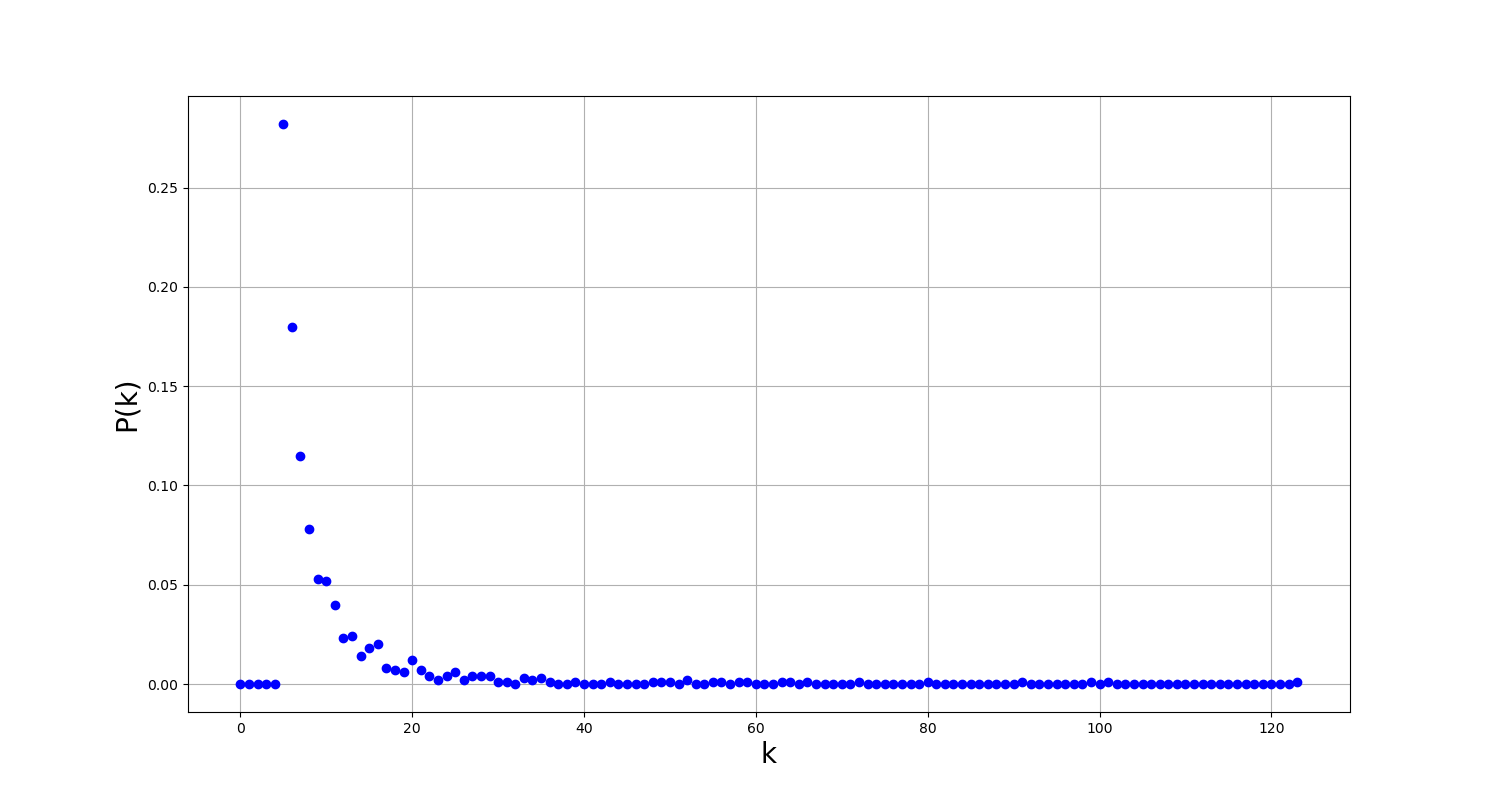
\includegraphics[width=18cm]{./Programming/degree-distribution.png}
        \caption{Degree Distribution}
        \label{fig3}
    \end{figure}
    \item[(b)] Compute $k_{nn}(k) = \E \left[ \sum_{i \in V} k_{nn, i} \delta_{k_i, k} / \sum_{i\in V} \delta_{k_i, k}\right]$ where $k_{nn, i} = \frac{1}{k_i} \sum_{j \in V} a_{ij} k_j$, and decide whether the graphs are typically uncorrelated or (dis-)assortative.
    
    \textit{ Sol. }

    \item[(c)] Plot the spectrum of the adjacency matrix $A = (a_{ij})$ using all realizations with a kernel density estimate, and compare it to the Wigner semi-circle law with $\sigma^2 = \Var [a_{ij}]$.
    
    \textit{ Sol. }

\end{enumerate}